\documentclass[1p]{elsarticle_modified}
%\bibliographystyle{elsarticle-num}

%\usepackage[colorlinks]{hyperref}
%\usepackage{abbrmath_seonhwa} %\Abb, \Ascr, \Acal ,\Abf, \Afrak
\usepackage{amsfonts}
\usepackage{amssymb}
\usepackage{amsmath}
\usepackage{amsthm}
\usepackage{scalefnt}
\usepackage{amsbsy}
\usepackage{kotex}
\usepackage{caption}
\usepackage{subfig}
\usepackage{color}
\usepackage{graphicx}
\usepackage{xcolor} %% white, black, red, green, blue, cyan, magenta, yellow
\usepackage{float}
\usepackage{setspace}
\usepackage{hyperref}

\usepackage{tikz}
\usetikzlibrary{arrows}

\usepackage{multirow}
\usepackage{array} % fixed length table
\usepackage{hhline}

%%%%%%%%%%%%%%%%%%%%%
\makeatletter
\renewcommand*\env@matrix[1][\arraystretch]{%
	\edef\arraystretch{#1}%
	\hskip -\arraycolsep
	\let\@ifnextchar\new@ifnextchar
	\array{*\c@MaxMatrixCols c}}
\makeatother %https://tex.stackexchange.com/questions/14071/how-can-i-increase-the-line-spacing-in-a-matrix
%%%%%%%%%%%%%%%

\usepackage[normalem]{ulem}

\newcommand{\msout}[1]{\ifmmode\text{\sout{\ensuremath{#1}}}\else\sout{#1}\fi}
%SOURCE: \msout is \stkout macro in https://tex.stackexchange.com/questions/20609/strikeout-in-math-mode

\newcommand{\cancel}[1]{
	\ifmmode
	{\color{red}\msout{#1}}
	\else
	{\color{red}\sout{#1}}
	\fi
}

\newcommand{\add}[1]{
	{\color{blue}\uwave{#1}}
}

\newcommand{\replace}[2]{
	\ifmmode
	{\color{red}\msout{#1}}{\color{blue}\uwave{#2}}
	\else
	{\color{red}\sout{#1}}{\color{blue}\uwave{#2}}
	\fi
}

\newcommand{\Sol}{\mathcal{S}} %segment
\newcommand{\D}{D} %diagram
\newcommand{\A}{\mathcal{A}} %arc


%%%%%%%%%%%%%%%%%%%%%%%%%%%%%5 test

\def\sl{\operatorname{\textup{SL}}(2,\Cbb)}
\def\psl{\operatorname{\textup{PSL}}(2,\Cbb)}
\def\quan{\mkern 1mu \triangleright \mkern 1mu}

\theoremstyle{definition}
\newtheorem{thm}{Theorem}[section]
\newtheorem{prop}[thm]{Proposition}
\newtheorem{lem}[thm]{Lemma}
\newtheorem{ques}[thm]{Question}
\newtheorem{cor}[thm]{Corollary}
\newtheorem{defn}[thm]{Definition}
\newtheorem{exam}[thm]{Example}
\newtheorem{rmk}[thm]{Remark}
\newtheorem{alg}[thm]{Algorithm}

\newcommand{\I}{\sqrt{-1}}
\begin{document}

%\begin{frontmatter}
%
%\title{Boundary parabolic representations of knots up to 8 crossings}
%
%%% Group authors per affiliation:
%\author{Yunhi Cho} 
%\address{Department of Mathematics, University of Seoul, Seoul, Korea}
%\ead{yhcho@uos.ac.kr}
%
%
%\author{Seonhwa Kim} %\fnref{s_kim}}
%\address{Center for Geometry and Physics, Institute for Basic Science, Pohang, 37673, Korea}
%\ead{ryeona17@ibs.re.kr}
%
%\author{Hyuk Kim}
%\address{Department of Mathematical Sciences, Seoul National University, Seoul 08826, Korea}
%\ead{hyukkim@snu.ac.kr}
%
%\author{Seokbeom Yoon}
%\address{Department of Mathematical Sciences, Seoul National University, Seoul, 08826,  Korea}
%\ead{sbyoon15@snu.ac.kr}
%
%\begin{abstract}
%We find all boundary parabolic representation of knots up to 8 crossings.
%
%\end{abstract}
%\begin{keyword}
%    \MSC[2010] 57M25 
%\end{keyword}
%
%\end{frontmatter}

%\linenumbers
%\tableofcontents
%
\newcommand\colored[1]{\textcolor{white}{\rule[-0.35ex]{0.8em}{1.4ex}}\kern-0.8em\color{red} #1}%
%\newcommand\colored[1]{\textcolor{white}{ #1}\kern-2.17ex	\textcolor{white}{ #1}\kern-1.81ex	\textcolor{white}{ #1}\kern-2.15ex\color{red}#1	}

{\Large $\underline{12n_{0220}~(K12n_{0220})}$}

\setlength{\tabcolsep}{10pt}
\renewcommand{\arraystretch}{1.6}
\vspace{1cm}\begin{tabular}{m{100pt}>{\centering\arraybackslash}m{274pt}}
\multirow{5}{120pt}{
	\centering
	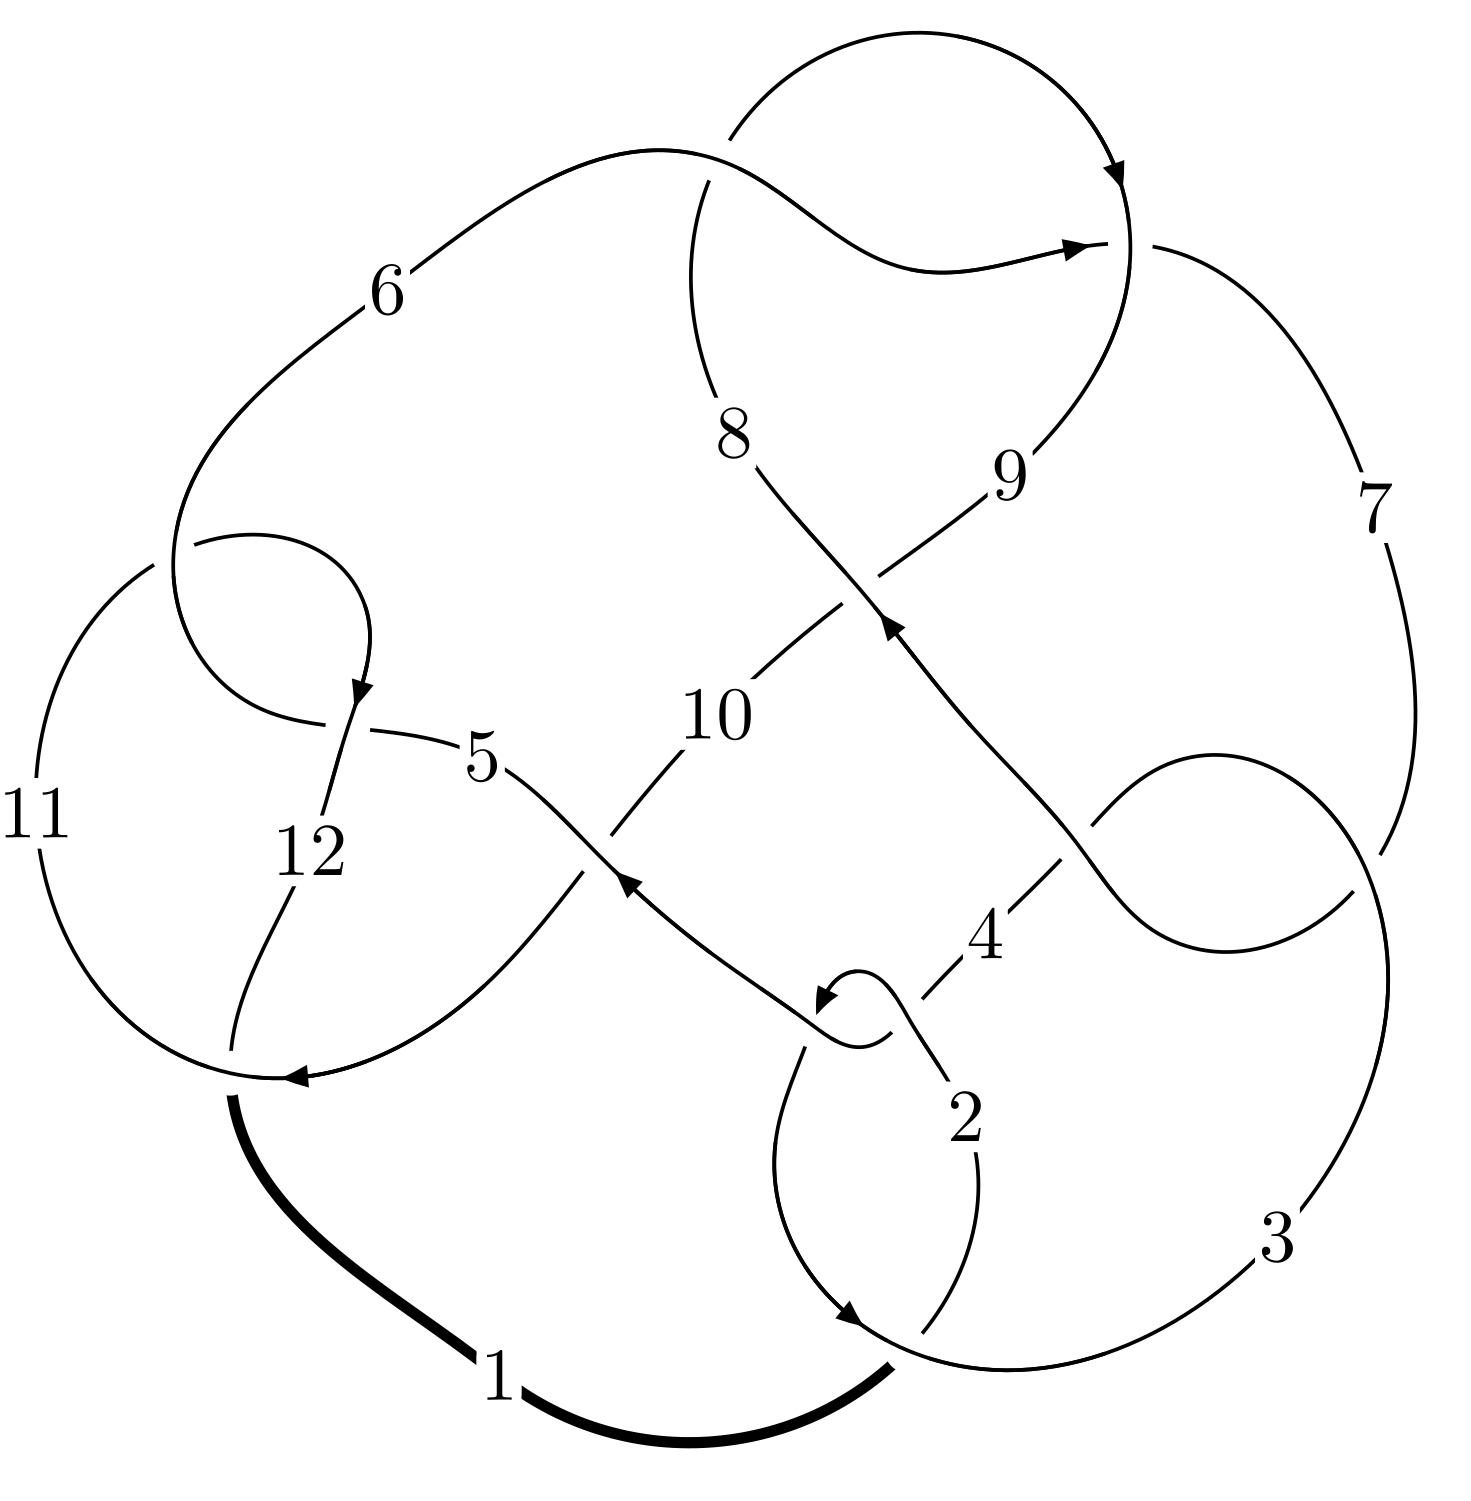
\includegraphics[width=112pt]{../../../GIT/diagram.site/Diagrams/png/2309_12n_0220.png}\\
\ \ \ A knot diagram\footnotemark}&
\allowdisplaybreaks
\textbf{Linearized knot diagam} \\
\cline{2-2}
 &
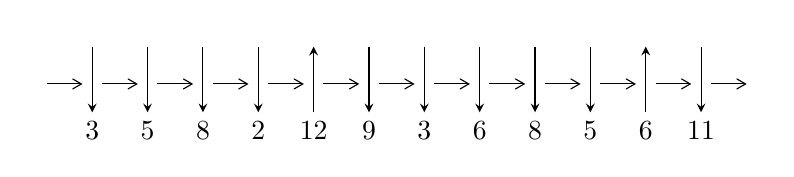
\begin{tikzpicture}[x=20pt, y=17pt]
	% nodes
	\node (C0) at (0, 0) {};
	\node (C1) at (1, 0) {};
	\node (C1U) at (1, +1) {};
	\node (C1D) at (1, -1) {3};

	\node (C2) at (2, 0) {};
	\node (C2U) at (2, +1) {};
	\node (C2D) at (2, -1) {5};

	\node (C3) at (3, 0) {};
	\node (C3U) at (3, +1) {};
	\node (C3D) at (3, -1) {8};

	\node (C4) at (4, 0) {};
	\node (C4U) at (4, +1) {};
	\node (C4D) at (4, -1) {2};

	\node (C5) at (5, 0) {};
	\node (C5U) at (5, +1) {};
	\node (C5D) at (5, -1) {12};

	\node (C6) at (6, 0) {};
	\node (C6U) at (6, +1) {};
	\node (C6D) at (6, -1) {9};

	\node (C7) at (7, 0) {};
	\node (C7U) at (7, +1) {};
	\node (C7D) at (7, -1) {3};

	\node (C8) at (8, 0) {};
	\node (C8U) at (8, +1) {};
	\node (C8D) at (8, -1) {6};

	\node (C9) at (9, 0) {};
	\node (C9U) at (9, +1) {};
	\node (C9D) at (9, -1) {8};

	\node (C10) at (10, 0) {};
	\node (C10U) at (10, +1) {};
	\node (C10D) at (10, -1) {5};

	\node (C11) at (11, 0) {};
	\node (C11U) at (11, +1) {};
	\node (C11D) at (11, -1) {6};

	\node (C12) at (12, 0) {};
	\node (C12U) at (12, +1) {};
	\node (C12D) at (12, -1) {11};
	\node (C13) at (13, 0) {};

	% arrows
	\draw[->,>={angle 60}]
	(C0) edge (C1) (C1) edge (C2) (C2) edge (C3) (C3) edge (C4) (C4) edge (C5) (C5) edge (C6) (C6) edge (C7) (C7) edge (C8) (C8) edge (C9) (C9) edge (C10) (C10) edge (C11) (C11) edge (C12) (C12) edge (C13) ;	\draw[->,>=stealth]
	(C1U) edge (C1D) (C2U) edge (C2D) (C3U) edge (C3D) (C4U) edge (C4D) (C5D) edge (C5U) (C6U) edge (C6D) (C7U) edge (C7D) (C8U) edge (C8D) (C9U) edge (C9D) (C10U) edge (C10D) (C11D) edge (C11U) (C12U) edge (C12D) ;
	\end{tikzpicture} \\
\hhline{~~} \\& 
\textbf{Solving Sequence} \\ \cline{2-2} 
 &
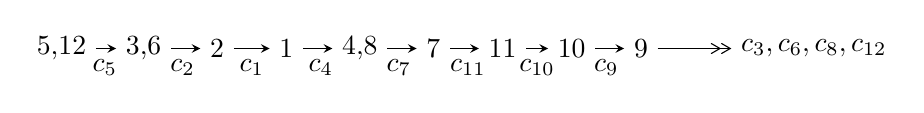
\begin{tikzpicture}[x=25pt, y=7pt]
	% node
	\node (A0) at (-1/8, 0) {5,12};
	\node (A1) at (17/16, 0) {3,6};
	\node (A2) at (17/8, 0) {2};
	\node (A3) at (25/8, 0) {1};
	\node (A4) at (67/16, 0) {4,8};
	\node (A5) at (21/4, 0) {7};
	\node (A6) at (25/4, 0) {11};
	\node (A7) at (29/4, 0) {10};
	\node (A8) at (33/4, 0) {9};
	\node (C1) at (1/2, -1) {$c_{5}$};
	\node (C2) at (13/8, -1) {$c_{2}$};
	\node (C3) at (21/8, -1) {$c_{1}$};
	\node (C4) at (29/8, -1) {$c_{4}$};
	\node (C5) at (19/4, -1) {$c_{7}$};
	\node (C6) at (23/4, -1) {$c_{11}$};
	\node (C7) at (27/4, -1) {$c_{10}$};
	\node (C8) at (31/4, -1) {$c_{9}$};
	\node (A9) at (43/4, 0) {$c_{3},c_{6},c_{8},c_{12}$};

	% edge
	\draw[->,>=stealth]	
	(A0) edge (A1) (A1) edge (A2) (A2) edge (A3) (A3) edge (A4) (A4) edge (A5) (A5) edge (A6) (A6) edge (A7) (A7) edge (A8) ;
	\draw[->>,>={angle 60}]	
	(A8) edge (A9);
\end{tikzpicture} \\ 

\end{tabular} \\

\footnotetext{
The image of knot diagram is generated by the software ``\textbf{Draw programme}" developed by Andrew Bartholomew(\url{http://www.layer8.co.uk/maths/draw/index.htm\#Running-draw}), where we modified some parts for our purpose(\url{https://github.com/CATsTAILs/LinksPainter}).
}\phantom \\ \newline 
\centering \textbf{Ideals for irreducible components\footnotemark of $X_{\text{par}}$} 
 
\begin{align*}
I^u_{1}&=\langle 
2281 u^{12}+1307 u^{11}+\cdots+44956 d+11490,\;1947 u^{12}+1293 u^{11}+\cdots+22478 c+16277,\\
\phantom{I^u_{1}}&\phantom{= \langle  }573 u^{12}+2043 u^{11}+\cdots+44956 b+16722,\;-1947 u^{12}-1293 u^{11}+\cdots+22478 a-16277,\\
\phantom{I^u_{1}}&\phantom{= \langle  }u^{13}+u^{12}+2 u^{11}+u^{10}+5 u^9+u^8+4 u^7+u^6+15 u^5+5 u^4+16 u^3+5 u^2+12 u+4\rangle \\
I^u_{2}&=\langle 
- u^4+u^2 a-2 u^3+a u- u^2+d+2 u+2,\;u^4+3 u^3+5 u^2+c- a+3 u+1,\;u^4+2 u^3- a u+2 u^2+b,\\
\phantom{I^u_{2}}&\phantom{= \langle  }- u^4 a-3 u^3 a+2 u^4-5 u^2 a+4 u^3+a^2-3 a u+3 u^2- a-2 u-1,\;u^5+2 u^4+2 u^3+u+1\rangle \\
I^u_{3}&=\langle 
d,\;c+u,\;b,\;a-1,\;u^2- u+1\rangle \\
I^u_{4}&=\langle 
d- u-1,\;c-1,\;b+1,\;a- u,\;u^2+u+1\rangle \\
I^u_{5}&=\langle 
- c u+d- c+1,\;c a- c u+a u,\;b+1,\;u^2+u+1\rangle \\
\\
I^v_{1}&=\langle 
a,\;d-1,\;c+a,\;b+1,\;v+1\rangle \\
\end{align*}
\raggedright * 5 irreducible components of $\dim_{\mathbb{C}}=0$, with total 28 representations.\\
\raggedright * 1 irreducible components of $\dim_{\mathbb{C}}=1$ \\
\footnotetext{All coefficients of polynomials are rational numbers. But the coefficients are sometimes approximated in decimal forms when there is not enough margin.}
\newpage
\renewcommand{\arraystretch}{1}
\centering \section*{I. $I^u_{1}= \langle 2281 u^{12}+1307 u^{11}+\cdots+4.50\times10^{4} d+1.15\times10^{4},\;1947 u^{12}+1293 u^{11}+\cdots+2.25\times10^{4} c+1.63\times10^{4},\;573 u^{12}+2043 u^{11}+\cdots+4.50\times10^{4} b+1.67\times10^{4},\;-1947 u^{12}-1293 u^{11}+\cdots+2.25\times10^{4} a-1.63\times10^{4},\;u^{13}+u^{12}+\cdots+12 u+4 \rangle$}
\flushleft \textbf{(i) Arc colorings}\\
\begin{tabular}{m{7pt} m{180pt} m{7pt} m{180pt} }
\flushright $a_{5}=$&$\begin{pmatrix}1\\0\end{pmatrix}$ \\
\flushright $a_{12}=$&$\begin{pmatrix}0\\u\end{pmatrix}$ \\
\flushright $a_{3}=$&$\begin{pmatrix}0.0866180 u^{12}+0.0575229 u^{11}+\cdots+0.482205 u+0.724130\\-0.0127458 u^{12}-0.0454444 u^{11}+\cdots+0.294221 u-0.371964\end{pmatrix}$ \\
\flushright $a_{6}=$&$\begin{pmatrix}1\\- u^2\end{pmatrix}$ \\
\flushright $a_{2}=$&$\begin{pmatrix}0.0738722 u^{12}+0.0120785 u^{11}+\cdots+0.776426 u+0.352167\\-0.0127458 u^{12}-0.0454444 u^{11}+\cdots+0.294221 u-0.371964\end{pmatrix}$ \\
\flushright $a_{1}=$&$\begin{pmatrix}- u^3\\u^5+u^3+u\end{pmatrix}$ \\
\flushright $a_{4}=$&$\begin{pmatrix}0.0683446 u^{12}-0.0285724 u^{11}+\cdots-0.389169 u+0.832214\\-0.00298069 u^{12}-0.0420411 u^{11}+\cdots-0.370985 u-0.374944\end{pmatrix}$ \\
\flushright $a_{8}=$&$\begin{pmatrix}-0.0866180 u^{12}-0.0575229 u^{11}+\cdots-0.482205 u-0.724130\\-0.0507385 u^{12}-0.0290729 u^{11}+\cdots+0.296890 u-0.255583\end{pmatrix}$ \\
\flushright $a_{7}=$&$\begin{pmatrix}-0.0683446 u^{12}+0.0285724 u^{11}+\cdots+0.389169 u-0.832214\\0.0180176 u^{12}-0.119005 u^{11}+\cdots+0.518640 u+0.0127236\end{pmatrix}$ \\
\flushright $a_{11}=$&$\begin{pmatrix}- u\\u^3+u\end{pmatrix}$ \\
\flushright $a_{10}=$&$\begin{pmatrix}u^3\\u^3+u\end{pmatrix}$ \\
\flushright $a_{9}=$&$\begin{pmatrix}-0.0738722 u^{12}-0.0120785 u^{11}+\cdots-0.776426 u-0.352167\\-0.0613266 u^{12}+0.0902438 u^{11}+\cdots+0.740257 u-0.124789\end{pmatrix}$\\&\end{tabular}
\flushleft \textbf{(ii) Obstruction class $= -1$}\\~\\
\flushleft \textbf{(iii) Cusp Shapes $= \frac{2015}{11239} u^{12}-\frac{4290}{11239} u^{11}+\cdots+\frac{6386}{11239} u-\frac{108192}{11239}$}\\~\\
\newpage\renewcommand{\arraystretch}{1}
\flushleft \textbf{(iv) u-Polynomials at the component}\newline \\
\begin{tabular}{m{50pt}|m{274pt}}
Crossings & \hspace{64pt}u-Polynomials at each crossing \\
\hline $$\begin{aligned}c_{1},c_{9}\end{aligned}$$&$\begin{aligned}
&u^{13}- u^{12}+\cdots+16 u+1
\end{aligned}$\\
\hline $$\begin{aligned}c_{2},c_{4},c_{6}\\c_{8}\end{aligned}$$&$\begin{aligned}
&u^{13}-5 u^{12}+\cdots-4 u+1
\end{aligned}$\\
\hline $$\begin{aligned}c_{3},c_{7}\end{aligned}$$&$\begin{aligned}
&u^{13}-3 u^{12}+\cdots-32 u+32
\end{aligned}$\\
\hline $$\begin{aligned}c_{5},c_{11}\end{aligned}$$&$\begin{aligned}
&u^{13}+u^{12}+\cdots+12 u+4
\end{aligned}$\\
\hline $$\begin{aligned}c_{10}\end{aligned}$$&$\begin{aligned}
&u^{13}- u^{12}+\cdots+1508 u+548
\end{aligned}$\\
\hline $$\begin{aligned}c_{12}\end{aligned}$$&$\begin{aligned}
&u^{13}+3 u^{12}+\cdots+104 u-16
\end{aligned}$\\
\hline
\end{tabular}\\~\\
\newpage\renewcommand{\arraystretch}{1}
\flushleft \textbf{(v) Riley Polynomials at the component}\newline \\
\begin{tabular}{m{50pt}|m{274pt}}
Crossings & \hspace{64pt}Riley Polynomials at each crossing \\
\hline $$\begin{aligned}c_{1},c_{9}\end{aligned}$$&$\begin{aligned}
&y^{13}+25 y^{12}+\cdots-260 y-1
\end{aligned}$\\
\hline $$\begin{aligned}c_{2},c_{4},c_{6}\\c_{8}\end{aligned}$$&$\begin{aligned}
&y^{13}+y^{12}+\cdots+16 y-1
\end{aligned}$\\
\hline $$\begin{aligned}c_{3},c_{7}\end{aligned}$$&$\begin{aligned}
&y^{13}+15 y^{12}+\cdots+15616 y^2-1024
\end{aligned}$\\
\hline $$\begin{aligned}c_{5},c_{11}\end{aligned}$$&$\begin{aligned}
&y^{13}+3 y^{12}+\cdots+104 y-16
\end{aligned}$\\
\hline $$\begin{aligned}c_{10}\end{aligned}$$&$\begin{aligned}
&y^{13}+27 y^{12}+\cdots+1970472 y-300304
\end{aligned}$\\
\hline $$\begin{aligned}c_{12}\end{aligned}$$&$\begin{aligned}
&y^{13}+15 y^{12}+\cdots+21024 y-256
\end{aligned}$\\
\hline
\end{tabular}\\~\\
\newpage\flushleft \textbf{(vi) Complex Volumes and Cusp Shapes}
$$\begin{array}{c|c|c}  
\text{Solutions to }I^u_{1}& \I (\text{vol} + \sqrt{-1}CS) & \text{Cusp shape}\\
 \hline 
\begin{aligned}
u &= -0.386403 + 0.917053 I \\
a &= -0.849710 + 0.767631 I \\
b &= -0.801603 - 0.173700 I \\
c &= \phantom{-}0.849710 - 0.767631 I \\
d &= \phantom{-}0.330147 - 0.102461 I\end{aligned}
 & -2.92013 - 2.62586 I & -15.8235 + 5.3570 I \\ \hline\begin{aligned}
u &= -0.386403 - 0.917053 I \\
a &= -0.849710 - 0.767631 I \\
b &= -0.801603 + 0.173700 I \\
c &= \phantom{-}0.849710 + 0.767631 I \\
d &= \phantom{-}0.330147 + 0.102461 I\end{aligned}
 & -2.92013 + 2.62586 I & -15.8235 - 5.3570 I \\ \hline\begin{aligned}
u &= \phantom{-}0.416573 + 0.881458 I \\
a &= \phantom{-}0.686659 + 0.124521 I \\
b &= \phantom{-}0.221947 + 0.150698 I \\
c &= -0.686659 - 0.124521 I \\
d &= -0.283854 + 0.579828 I\end{aligned}
 & -0.33676 + 1.74909 I & -2.22256 - 3.20069 I \\ \hline\begin{aligned}
u &= \phantom{-}0.416573 - 0.881458 I \\
a &= \phantom{-}0.686659 - 0.124521 I \\
b &= \phantom{-}0.221947 - 0.150698 I \\
c &= -0.686659 + 0.124521 I \\
d &= -0.283854 - 0.579828 I\end{aligned}
 & -0.33676 - 1.74909 I & -2.22256 + 3.20069 I \\ \hline\begin{aligned}
u &= \phantom{-}1.124080 + 0.602862 I \\
a &= -0.176205 - 1.075190 I \\
b &= -0.16802 + 1.50582 I \\
c &= \phantom{-}0.176205 + 1.075190 I \\
d &= \phantom{-}1.130610 + 0.299207 I\end{aligned}
 & \phantom{-}4.55733 + 1.91344 I & -6.23694 - 1.74226 I \\ \hline\begin{aligned}
u &= \phantom{-}1.124080 - 0.602862 I \\
a &= -0.176205 + 1.075190 I \\
b &= -0.16802 - 1.50582 I \\
c &= \phantom{-}0.176205 - 1.075190 I \\
d &= \phantom{-}1.130610 - 0.299207 I\end{aligned}
 & \phantom{-}4.55733 - 1.91344 I & -6.23694 + 1.74226 I\\
 \hline 
 \end{array}$$\newpage$$\begin{array}{c|c|c}  
\text{Solutions to }I^u_{1}& \I (\text{vol} + \sqrt{-1}CS) & \text{Cusp shape}\\
 \hline 
\begin{aligned}
u &= \phantom{-}0.543511 + 1.275200 I \\
a &= \phantom{-}1.113650 + 0.332769 I \\
b &= \phantom{-}0.536277 - 1.193890 I \\
c &= -1.113650 - 0.332769 I \\
d &= -1.406970 - 0.093004 I\end{aligned}
 & \phantom{-}1.88235 + 4.50009 I & -8.08386 - 3.64476 I \\ \hline\begin{aligned}
u &= \phantom{-}0.543511 - 1.275200 I \\
a &= \phantom{-}1.113650 - 0.332769 I \\
b &= \phantom{-}0.536277 + 1.193890 I \\
c &= -1.113650 + 0.332769 I \\
d &= -1.406970 + 0.093004 I\end{aligned}
 & \phantom{-}1.88235 - 4.50009 I & -8.08386 + 3.64476 I \\ \hline\begin{aligned}
u &= -1.173290 + 0.753740 I \\
a &= -0.464126 + 0.518194 I \\
b &= \phantom{-}1.48175 - 1.16585 I \\
c &= \phantom{-}0.464126 - 0.518194 I \\
d &= \phantom{-}2.02304 + 0.07401 I\end{aligned}
 & \phantom{-}13.3607 + 6.1261 I & -8.08998 - 1.87384 I \\ \hline\begin{aligned}
u &= -1.173290 - 0.753740 I \\
a &= -0.464126 - 0.518194 I \\
b &= \phantom{-}1.48175 + 1.16585 I \\
c &= \phantom{-}0.464126 + 0.518194 I \\
d &= \phantom{-}2.02304 - 0.07401 I\end{aligned}
 & \phantom{-}13.3607 - 6.1261 I & -8.08998 + 1.87384 I \\ \hline\begin{aligned}
u &= -0.85913 + 1.17284 I \\
a &= \phantom{-}0.84945 - 1.49776 I \\
b &= \phantom{-}1.47195 + 0.93931 I \\
c &= -0.84945 + 1.49776 I \\
d &= -2.08790 + 0.18218 I\end{aligned}
 & \phantom{-}11.8885 - 13.4346 I & -9.57192 + 6.10692 I \\ \hline\begin{aligned}
u &= -0.85913 - 1.17284 I \\
a &= \phantom{-}0.84945 + 1.49776 I \\
b &= \phantom{-}1.47195 - 0.93931 I \\
c &= -0.84945 - 1.49776 I \\
d &= -2.08790 - 0.18218 I\end{aligned}
 & \phantom{-}11.8885 + 13.4346 I & -9.57192 - 6.10692 I\\
 \hline 
 \end{array}$$\newpage$$\begin{array}{c|c|c}  
\text{Solutions to }I^u_{1}& \I (\text{vol} + \sqrt{-1}CS) & \text{Cusp shape}\\
 \hline 
\begin{aligned}
u &= -0.330680\phantom{ +0.000000I} \\
a &= \phantom{-}0.680555\phantom{ +0.000000I} \\
b &= -0.484585\phantom{ +0.000000I} \\
c &= -0.680555\phantom{ +0.000000I} \\
d &= -0.410167\phantom{ +0.000000I}\end{aligned}
 & -0.936151\phantom{ +0.000000I} & -9.94250\phantom{ +0.000000I}\\
 \hline 
 \end{array}$$\newpage\newpage\renewcommand{\arraystretch}{1}
\centering \section*{II. $I^u_{2}= \langle - u^4-2 u^3+\cdots+d+2,\;u^4+3 u^3+\cdots- a+1,\;u^4+2 u^3- a u+2 u^2+b,\;- u^4 a+2 u^4+\cdots- a-1,\;u^5+2 u^4+2 u^3+u+1 \rangle$}
\flushleft \textbf{(i) Arc colorings}\\
\begin{tabular}{m{7pt} m{180pt} m{7pt} m{180pt} }
\flushright $a_{5}=$&$\begin{pmatrix}1\\0\end{pmatrix}$ \\
\flushright $a_{12}=$&$\begin{pmatrix}0\\u\end{pmatrix}$ \\
\flushright $a_{3}=$&$\begin{pmatrix}a\\- u^4-2 u^3+a u-2 u^2\end{pmatrix}$ \\
\flushright $a_{6}=$&$\begin{pmatrix}1\\- u^2\end{pmatrix}$ \\
\flushright $a_{2}=$&$\begin{pmatrix}- u^4-2 u^3+a u-2 u^2+a\\- u^4-2 u^3+a u-2 u^2\end{pmatrix}$ \\
\flushright $a_{1}=$&$\begin{pmatrix}- u^3\\-2 u^4- u^3-1\end{pmatrix}$ \\
\flushright $a_{4}=$&$\begin{pmatrix}- u^4 a-2 u^3 a- u^2 a- u^2-3 u-1\\- u^4 a- u^3 a+u^3+u^2- a\end{pmatrix}$ \\
\flushright $a_{8}=$&$\begin{pmatrix}- u^4-3 u^3-5 u^2+a-3 u-1\\u^4- u^2 a+2 u^3- a u+u^2-2 u-2\end{pmatrix}$ \\
\flushright $a_{7}=$&$\begin{pmatrix}- u^4 a-2 u^3 a- u^4- u^2 a-3 u^3-5 u^2-3 u-1\\u^3 a+u^4- u^2 a+u^3- a u+a-3 u-2\end{pmatrix}$ \\
\flushright $a_{11}=$&$\begin{pmatrix}- u\\u^3+u\end{pmatrix}$ \\
\flushright $a_{10}=$&$\begin{pmatrix}u^3\\u^3+u\end{pmatrix}$ \\
\flushright $a_{9}=$&$\begin{pmatrix}- u^4-4 u^3+a u-6 u^2+a-3 u\\- u^3 a- u^2 a- a u-3 u-3\end{pmatrix}$\\&\end{tabular}
\flushleft \textbf{(ii) Obstruction class $= -1$}\\~\\
\flushleft \textbf{(iii) Cusp Shapes $= u^4+u^3-2 u^2-5 u-10$}\\~\\
\newpage\renewcommand{\arraystretch}{1}
\flushleft \textbf{(iv) u-Polynomials at the component}\newline \\
\begin{tabular}{m{50pt}|m{274pt}}
Crossings & \hspace{64pt}u-Polynomials at each crossing \\
\hline $$\begin{aligned}c_{1},c_{9}\end{aligned}$$&$\begin{aligned}
&u^{10}- u^9+\cdots+800 u+256
\end{aligned}$\\
\hline $$\begin{aligned}c_{2},c_{4},c_{6}\\c_{8}\end{aligned}$$&$\begin{aligned}
&u^{10}-3 u^9+5 u^8+3 u^7-12 u^6+10 u^5+17 u^4-18 u^3-23 u^2+8 u+16
\end{aligned}$\\
\hline $$\begin{aligned}c_{3},c_{7}\end{aligned}$$&$\begin{aligned}
&(u^5+u^4+8 u^3+u^2-4 u+4)^2
\end{aligned}$\\
\hline $$\begin{aligned}c_{5},c_{11}\end{aligned}$$&$\begin{aligned}
&(u^5+2 u^4+2 u^3+u+1)^2
\end{aligned}$\\
\hline $$\begin{aligned}c_{10}\end{aligned}$$&$\begin{aligned}
&(u^5-2 u^4+14 u^3+16 u^2+9 u+9)^2
\end{aligned}$\\
\hline $$\begin{aligned}c_{12}\end{aligned}$$&$\begin{aligned}
&(u^5+6 u^3+u-1)^2
\end{aligned}$\\
\hline
\end{tabular}\\~\\
\newpage\renewcommand{\arraystretch}{1}
\flushleft \textbf{(v) Riley Polynomials at the component}\newline \\
\begin{tabular}{m{50pt}|m{274pt}}
Crossings & \hspace{64pt}Riley Polynomials at each crossing \\
\hline $$\begin{aligned}c_{1},c_{9}\end{aligned}$$&$\begin{aligned}
&y^{10}+37 y^9+\cdots+56832 y+65536
\end{aligned}$\\
\hline $$\begin{aligned}c_{2},c_{4},c_{6}\\c_{8}\end{aligned}$$&$\begin{aligned}
&y^{10}+y^9+\cdots-800 y+256
\end{aligned}$\\
\hline $$\begin{aligned}c_{3},c_{7}\end{aligned}$$&$\begin{aligned}
&(y^5+15 y^4+54 y^3-73 y^2+8 y-16)^2
\end{aligned}$\\
\hline $$\begin{aligned}c_{5},c_{11}\end{aligned}$$&$\begin{aligned}
&(y^5+6 y^3+y-1)^2
\end{aligned}$\\
\hline $$\begin{aligned}c_{10}\end{aligned}$$&$\begin{aligned}
&(y^5+24 y^4+278 y^3+32 y^2-207 y-81)^2
\end{aligned}$\\
\hline $$\begin{aligned}c_{12}\end{aligned}$$&$\begin{aligned}
&(y^5+12 y^4+38 y^3+12 y^2+y-1)^2
\end{aligned}$\\
\hline
\end{tabular}\\~\\
\newpage\flushleft \textbf{(vi) Complex Volumes and Cusp Shapes}
$$\begin{array}{c|c|c}  
\text{Solutions to }I^u_{2}& \I (\text{vol} + \sqrt{-1}CS) & \text{Cusp shape}\\
 \hline 
\begin{aligned}
u &= \phantom{-}0.436447 + 0.655029 I \\
a &= \phantom{-}0.445445 + 1.296420 I \\
b &= \phantom{-}1.049680 - 0.199668 I \\
c &= \phantom{-}1.03494 - 3.53452 I \\
d &= -2.83647 - 1.62756 I\end{aligned}
 & -3.34738 + 1.37362 I & -12.45374 - 4.59823 I \\ \hline\begin{aligned}
u &= \phantom{-}0.436447 + 0.655029 I \\
a &= -1.03494 + 3.53452 I \\
b &= -1.062450 - 0.192555 I \\
c &= -0.445445 - 1.296420 I \\
d &= \phantom{-}0.202150 - 0.254271 I\end{aligned}
 & -3.34738 + 1.37362 I & -12.45374 - 4.59823 I \\ \hline\begin{aligned}
u &= \phantom{-}0.436447 - 0.655029 I \\
a &= \phantom{-}0.445445 - 1.296420 I \\
b &= \phantom{-}1.049680 + 0.199668 I \\
c &= \phantom{-}1.03494 + 3.53452 I \\
d &= -2.83647 + 1.62756 I\end{aligned}
 & -3.34738 - 1.37362 I & -12.45374 + 4.59823 I \\ \hline\begin{aligned}
u &= \phantom{-}0.436447 - 0.655029 I \\
a &= -1.03494 - 3.53452 I \\
b &= -1.062450 + 0.192555 I \\
c &= -0.445445 + 1.296420 I \\
d &= \phantom{-}0.202150 + 0.254271 I\end{aligned}
 & -3.34738 - 1.37362 I & -12.45374 + 4.59823 I \\ \hline\begin{aligned}
u &= -0.668466\phantom{ +0.000000I} \\
a &= \phantom{-}0.266201 + 0.900637 I \\
b &= -0.673909 - 0.602045 I \\
c &= -0.266201 + 0.900637 I \\
d &= -0.554957 + 0.199598 I\end{aligned}
 & -0.737094\phantom{ +0.000000I} & -7.65040\phantom{ +0.000000I} \\ \hline\begin{aligned}
u &= -0.668466\phantom{ +0.000000I} \\
a &= \phantom{-}0.266201 - 0.900637 I \\
b &= -0.673909 + 0.602045 I \\
c &= -0.266201 - 0.900637 I \\
d &= -0.554957 - 0.199598 I\end{aligned}
 & -0.737094\phantom{ +0.000000I} & -7.65040\phantom{ +0.000000I}\\
 \hline 
 \end{array}$$\newpage$$\begin{array}{c|c|c}  
\text{Solutions to }I^u_{2}& \I (\text{vol} + \sqrt{-1}CS) & \text{Cusp shape}\\
 \hline 
\begin{aligned}
u &= -1.10221 + 1.09532 I \\
a &= -0.730929 + 0.410318 I \\
b &= \phantom{-}0.89973 - 1.70648 I \\
c &= -0.554227 + 1.236440 I \\
d &= -1.69011 + 0.15931 I\end{aligned}
 & \phantom{-}14.4080 - 4.0569 I & -7.72106 + 1.95729 I \\ \hline\begin{aligned}
u &= -1.10221 + 1.09532 I \\
a &= \phantom{-}0.554227 - 1.236440 I \\
b &= \phantom{-}1.28694 + 1.51626 I \\
c &= \phantom{-}0.730929 - 0.410318 I \\
d &= \phantom{-}1.87939 + 0.06460 I\end{aligned}
 & \phantom{-}14.4080 - 4.0569 I & -7.72106 + 1.95729 I \\ \hline\begin{aligned}
u &= -1.10221 - 1.09532 I \\
a &= -0.730929 - 0.410318 I \\
b &= \phantom{-}0.89973 + 1.70648 I \\
c &= -0.554227 - 1.236440 I \\
d &= -1.69011 - 0.15931 I\end{aligned}
 & \phantom{-}14.4080 + 4.0569 I & -7.72106 - 1.95729 I \\ \hline\begin{aligned}
u &= -1.10221 - 1.09532 I \\
a &= \phantom{-}0.554227 + 1.236440 I \\
b &= \phantom{-}1.28694 - 1.51626 I \\
c &= \phantom{-}0.730929 + 0.410318 I \\
d &= \phantom{-}1.87939 - 0.06460 I\end{aligned}
 & \phantom{-}14.4080 + 4.0569 I & -7.72106 - 1.95729 I\\
 \hline 
 \end{array}$$\newpage\newpage\renewcommand{\arraystretch}{1}
\centering \section*{III. $I^u_{3}= \langle d,\;c+u,\;b,\;a-1,\;u^2- u+1 \rangle$}
\flushleft \textbf{(i) Arc colorings}\\
\begin{tabular}{m{7pt} m{180pt} m{7pt} m{180pt} }
\flushright $a_{5}=$&$\begin{pmatrix}1\\0\end{pmatrix}$ \\
\flushright $a_{12}=$&$\begin{pmatrix}0\\u\end{pmatrix}$ \\
\flushright $a_{3}=$&$\begin{pmatrix}1\\0\end{pmatrix}$ \\
\flushright $a_{6}=$&$\begin{pmatrix}1\\- u+1\end{pmatrix}$ \\
\flushright $a_{2}=$&$\begin{pmatrix}1\\0\end{pmatrix}$ \\
\flushright $a_{1}=$&$\begin{pmatrix}1\\0\end{pmatrix}$ \\
\flushright $a_{4}=$&$\begin{pmatrix}1\\0\end{pmatrix}$ \\
\flushright $a_{8}=$&$\begin{pmatrix}- u\\0\end{pmatrix}$ \\
\flushright $a_{7}=$&$\begin{pmatrix}- u\\0\end{pmatrix}$ \\
\flushright $a_{11}=$&$\begin{pmatrix}- u\\u-1\end{pmatrix}$ \\
\flushright $a_{10}=$&$\begin{pmatrix}-1\\u-1\end{pmatrix}$ \\
\flushright $a_{9}=$&$\begin{pmatrix}- u-1\\u-1\end{pmatrix}$\\&\end{tabular}
\flushleft \textbf{(ii) Obstruction class $= 1$}\\~\\
\flushleft \textbf{(iii) Cusp Shapes $= -4 u-7$}\\~\\
\newpage\renewcommand{\arraystretch}{1}
\flushleft \textbf{(iv) u-Polynomials at the component}\newline \\
\begin{tabular}{m{50pt}|m{274pt}}
Crossings & \hspace{64pt}u-Polynomials at each crossing \\
\hline $$\begin{aligned}c_{1},c_{2},c_{3}\\c_{4},c_{7}\end{aligned}$$&$\begin{aligned}
&u^2
\end{aligned}$\\
\hline $$\begin{aligned}c_{5},c_{10}\end{aligned}$$&$\begin{aligned}
&u^2- u+1
\end{aligned}$\\
\hline $$\begin{aligned}c_{6}\end{aligned}$$&$\begin{aligned}
&(u-1)^2
\end{aligned}$\\
\hline $$\begin{aligned}c_{8},c_{9}\end{aligned}$$&$\begin{aligned}
&(u+1)^2
\end{aligned}$\\
\hline $$\begin{aligned}c_{11},c_{12}\end{aligned}$$&$\begin{aligned}
&u^2+u+1
\end{aligned}$\\
\hline
\end{tabular}\\~\\
\newpage\renewcommand{\arraystretch}{1}
\flushleft \textbf{(v) Riley Polynomials at the component}\newline \\
\begin{tabular}{m{50pt}|m{274pt}}
Crossings & \hspace{64pt}Riley Polynomials at each crossing \\
\hline $$\begin{aligned}c_{1},c_{2},c_{3}\\c_{4},c_{7}\end{aligned}$$&$\begin{aligned}
&y^2
\end{aligned}$\\
\hline $$\begin{aligned}c_{5},c_{10},c_{11}\\c_{12}\end{aligned}$$&$\begin{aligned}
&y^2+y+1
\end{aligned}$\\
\hline $$\begin{aligned}c_{6},c_{8},c_{9}\end{aligned}$$&$\begin{aligned}
&(y-1)^2
\end{aligned}$\\
\hline
\end{tabular}\\~\\
\newpage\flushleft \textbf{(vi) Complex Volumes and Cusp Shapes}
$$\begin{array}{c|c|c}  
\text{Solutions to }I^u_{3}& \I (\text{vol} + \sqrt{-1}CS) & \text{Cusp shape}\\
 \hline 
\begin{aligned}
u &= \phantom{-}0.500000 + 0.866025 I \\
a &= \phantom{-}1.00000\phantom{ +0.000000I} \\
b &= \phantom{-0.000000 } 0 \\
c &= -0.500000 - 0.866025 I \\
d &= \phantom{-0.000000 } 0\end{aligned}
 & -1.64493 + 2.02988 I & -9.00000 - 3.46410 I \\ \hline\begin{aligned}
u &= \phantom{-}0.500000 - 0.866025 I \\
a &= \phantom{-}1.00000\phantom{ +0.000000I} \\
b &= \phantom{-0.000000 } 0 \\
c &= -0.500000 + 0.866025 I \\
d &= \phantom{-0.000000 } 0\end{aligned}
 & -1.64493 - 2.02988 I & -9.00000 + 3.46410 I\\
 \hline 
 \end{array}$$\newpage\newpage\renewcommand{\arraystretch}{1}
\centering \section*{IV. $I^u_{4}= \langle d- u-1,\;c-1,\;b+1,\;a- u,\;u^2+u+1 \rangle$}
\flushleft \textbf{(i) Arc colorings}\\
\begin{tabular}{m{7pt} m{180pt} m{7pt} m{180pt} }
\flushright $a_{5}=$&$\begin{pmatrix}1\\0\end{pmatrix}$ \\
\flushright $a_{12}=$&$\begin{pmatrix}0\\u\end{pmatrix}$ \\
\flushright $a_{3}=$&$\begin{pmatrix}u\\-1\end{pmatrix}$ \\
\flushright $a_{6}=$&$\begin{pmatrix}1\\u+1\end{pmatrix}$ \\
\flushright $a_{2}=$&$\begin{pmatrix}u-1\\-1\end{pmatrix}$ \\
\flushright $a_{1}=$&$\begin{pmatrix}-1\\0\end{pmatrix}$ \\
\flushright $a_{4}=$&$\begin{pmatrix}u\\-1\end{pmatrix}$ \\
\flushright $a_{8}=$&$\begin{pmatrix}1\\u+1\end{pmatrix}$ \\
\flushright $a_{7}=$&$\begin{pmatrix}1\\u+1\end{pmatrix}$ \\
\flushright $a_{11}=$&$\begin{pmatrix}- u\\u+1\end{pmatrix}$ \\
\flushright $a_{10}=$&$\begin{pmatrix}1\\u+1\end{pmatrix}$ \\
\flushright $a_{9}=$&$\begin{pmatrix}1\\u+1\end{pmatrix}$\\&\end{tabular}
\flushleft \textbf{(ii) Obstruction class $= 1$}\\~\\
\flushleft \textbf{(iii) Cusp Shapes $= 4 u-7$}\\~\\
\newpage\renewcommand{\arraystretch}{1}
\flushleft \textbf{(iv) u-Polynomials at the component}\newline \\
\begin{tabular}{m{50pt}|m{274pt}}
Crossings & \hspace{64pt}u-Polynomials at each crossing \\
\hline $$\begin{aligned}c_{1},c_{2}\end{aligned}$$&$\begin{aligned}
&(u-1)^2
\end{aligned}$\\
\hline $$\begin{aligned}c_{3},c_{6},c_{7}\\c_{8},c_{9}\end{aligned}$$&$\begin{aligned}
&u^2
\end{aligned}$\\
\hline $$\begin{aligned}c_{4}\end{aligned}$$&$\begin{aligned}
&(u+1)^2
\end{aligned}$\\
\hline $$\begin{aligned}c_{5},c_{10},c_{12}\end{aligned}$$&$\begin{aligned}
&u^2+u+1
\end{aligned}$\\
\hline $$\begin{aligned}c_{11}\end{aligned}$$&$\begin{aligned}
&u^2- u+1
\end{aligned}$\\
\hline
\end{tabular}\\~\\
\newpage\renewcommand{\arraystretch}{1}
\flushleft \textbf{(v) Riley Polynomials at the component}\newline \\
\begin{tabular}{m{50pt}|m{274pt}}
Crossings & \hspace{64pt}Riley Polynomials at each crossing \\
\hline $$\begin{aligned}c_{1},c_{2},c_{4}\end{aligned}$$&$\begin{aligned}
&(y-1)^2
\end{aligned}$\\
\hline $$\begin{aligned}c_{3},c_{6},c_{7}\\c_{8},c_{9}\end{aligned}$$&$\begin{aligned}
&y^2
\end{aligned}$\\
\hline $$\begin{aligned}c_{5},c_{10},c_{11}\\c_{12}\end{aligned}$$&$\begin{aligned}
&y^2+y+1
\end{aligned}$\\
\hline
\end{tabular}\\~\\
\newpage\flushleft \textbf{(vi) Complex Volumes and Cusp Shapes}
$$\begin{array}{c|c|c}  
\text{Solutions to }I^u_{4}& \I (\text{vol} + \sqrt{-1}CS) & \text{Cusp shape}\\
 \hline 
\begin{aligned}
u &= -0.500000 + 0.866025 I \\
a &= -0.500000 + 0.866025 I \\
b &= -1.00000\phantom{ +0.000000I} \\
c &= \phantom{-}1.00000\phantom{ +0.000000I} \\
d &= \phantom{-}0.500000 + 0.866025 I\end{aligned}
 & -1.64493 - 2.02988 I & -9.00000 + 3.46410 I \\ \hline\begin{aligned}
u &= -0.500000 - 0.866025 I \\
a &= -0.500000 - 0.866025 I \\
b &= -1.00000\phantom{ +0.000000I} \\
c &= \phantom{-}1.00000\phantom{ +0.000000I} \\
d &= \phantom{-}0.500000 - 0.866025 I\end{aligned}
 & -1.64493 + 2.02988 I & -9.00000 - 3.46410 I\\
 \hline 
 \end{array}$$\newpage\newpage\renewcommand{\arraystretch}{1}
\centering \section*{V. $I^u_{5}= \langle - c u+d- c+1,\;c a- c u+a u,\;b+1,\;u^2+u+1 \rangle$}
\flushleft \textbf{(i) Arc colorings}\\
\begin{tabular}{m{7pt} m{180pt} m{7pt} m{180pt} }
\flushright $a_{5}=$&$\begin{pmatrix}1\\0\end{pmatrix}$ \\
\flushright $a_{12}=$&$\begin{pmatrix}0\\u\end{pmatrix}$ \\
\flushright $a_{3}=$&$\begin{pmatrix}a\\-1\end{pmatrix}$ \\
\flushright $a_{6}=$&$\begin{pmatrix}1\\u+1\end{pmatrix}$ \\
\flushright $a_{2}=$&$\begin{pmatrix}a-1\\-1\end{pmatrix}$ \\
\flushright $a_{1}=$&$\begin{pmatrix}-1\\0\end{pmatrix}$ \\
\flushright $a_{4}=$&$\begin{pmatrix}a\\-1\end{pmatrix}$ \\
\flushright $a_{8}=$&$\begin{pmatrix}c\\c u+c-1\end{pmatrix}$ \\
\flushright $a_{7}=$&$\begin{pmatrix}c\\c u+c-1\end{pmatrix}$ \\
\flushright $a_{11}=$&$\begin{pmatrix}- u\\u+1\end{pmatrix}$ \\
\flushright $a_{10}=$&$\begin{pmatrix}1\\u+1\end{pmatrix}$ \\
\flushright $a_{9}=$&$\begin{pmatrix}c+1\\c u+c+u\end{pmatrix}$\\&\end{tabular}
\flushleft \textbf{(ii) Obstruction class $= -1$}\\~\\
\flushleft \textbf{(iii) Cusp Shapes $= c^2 u+a^2 u-2 c u+2 a u-2 c+2 a+4 u-10$}\\~\\
\flushleft \textbf{(iv) u-Polynomials at the component} : It cannot be defined for a positive dimension component.\\~\\
\flushleft \textbf{(v) Riley Polynomials at the component} : It cannot be defined for a positive dimension component.\\~\\
\newpage\flushleft \textbf{(iv) Complex Volumes and Cusp Shapes}
$$\begin{array}{c|c|c} 
\text{Solution to }I^u_{5}& \I (\text{vol} + \sqrt{-1}CS) & \text{Cusp shape}\\
 \hline 
\begin{aligned}
u &= \cdots \\
a &= \cdots \\
b &= \cdots \\
c &= \cdots \\
d &= \cdots\end{aligned}
 & -3.28987 + 2.02988 I & -13.6251 - 6.4182 I\\
 \hline 
 \end{array}
$$\newpage\renewcommand{\arraystretch}{1}
\centering \section*{VI. $I^v_{1}= \langle a,\;d-1,\;c+a,\;b+1,\;v+1 \rangle$}
\flushleft \textbf{(i) Arc colorings}\\
\begin{tabular}{m{7pt} m{180pt} m{7pt} m{180pt} }
\flushright $a_{5}=$&$\begin{pmatrix}1\\0\end{pmatrix}$ \\
\flushright $a_{12}=$&$\begin{pmatrix}-1\\0\end{pmatrix}$ \\
\flushright $a_{3}=$&$\begin{pmatrix}0\\-1\end{pmatrix}$ \\
\flushright $a_{6}=$&$\begin{pmatrix}1\\0\end{pmatrix}$ \\
\flushright $a_{2}=$&$\begin{pmatrix}-1\\-1\end{pmatrix}$ \\
\flushright $a_{1}=$&$\begin{pmatrix}-1\\0\end{pmatrix}$ \\
\flushright $a_{4}=$&$\begin{pmatrix}0\\-1\end{pmatrix}$ \\
\flushright $a_{8}=$&$\begin{pmatrix}0\\1\end{pmatrix}$ \\
\flushright $a_{7}=$&$\begin{pmatrix}0\\1\end{pmatrix}$ \\
\flushright $a_{11}=$&$\begin{pmatrix}-1\\0\end{pmatrix}$ \\
\flushright $a_{10}=$&$\begin{pmatrix}-1\\0\end{pmatrix}$ \\
\flushright $a_{9}=$&$\begin{pmatrix}-1\\1\end{pmatrix}$\\&\end{tabular}
\flushleft \textbf{(ii) Obstruction class $= 1$}\\~\\
\flushleft \textbf{(iii) Cusp Shapes $= -12$}\\~\\
\newpage\renewcommand{\arraystretch}{1}
\flushleft \textbf{(iv) u-Polynomials at the component}\newline \\
\begin{tabular}{m{50pt}|m{274pt}}
Crossings & \hspace{64pt}u-Polynomials at each crossing \\
\hline $$\begin{aligned}c_{1},c_{2},c_{6}\end{aligned}$$&$\begin{aligned}
&u-1
\end{aligned}$\\
\hline $$\begin{aligned}c_{3},c_{5},c_{7}\\c_{10},c_{11},c_{12}\end{aligned}$$&$\begin{aligned}
&u
\end{aligned}$\\
\hline $$\begin{aligned}c_{4},c_{8},c_{9}\end{aligned}$$&$\begin{aligned}
&u+1
\end{aligned}$\\
\hline
\end{tabular}\\~\\
\newpage\renewcommand{\arraystretch}{1}
\flushleft \textbf{(v) Riley Polynomials at the component}\newline \\
\begin{tabular}{m{50pt}|m{274pt}}
Crossings & \hspace{64pt}Riley Polynomials at each crossing \\
\hline $$\begin{aligned}c_{1},c_{2},c_{4}\\c_{6},c_{8},c_{9}\end{aligned}$$&$\begin{aligned}
&y-1
\end{aligned}$\\
\hline $$\begin{aligned}c_{3},c_{5},c_{7}\\c_{10},c_{11},c_{12}\end{aligned}$$&$\begin{aligned}
&y
\end{aligned}$\\
\hline
\end{tabular}\\~\\
\newpage\flushleft \textbf{(vi) Complex Volumes and Cusp Shapes}
$$\begin{array}{c|c|c}  
\text{Solutions to }I^v_{1}& \I (\text{vol} + \sqrt{-1}CS) & \text{Cusp shape}\\
 \hline 
\begin{aligned}
v &= -1.00000\phantom{ +0.000000I} \\
a &= \phantom{-0.000000 } 0 \\
b &= -1.00000\phantom{ +0.000000I} \\
c &= \phantom{-0.000000 } 0 \\
d &= \phantom{-}1.00000\phantom{ +0.000000I}\end{aligned}
 & -3.28987\phantom{ +0.000000I} & -12.0000\phantom{ +0.000000I}\\
 \hline 
 \end{array}$$\newpage
\newpage\renewcommand{\arraystretch}{1}
\centering \section*{ VII. u-Polynomials}
\begin{tabular}{m{50pt}|m{274pt}}
Crossings & \hspace{64pt}u-Polynomials at each crossing \\
\hline $$\begin{aligned}c_{1}\end{aligned}$$&$\begin{aligned}
&u^2(u-1)^3(u^{10}-u^{9}+\cdots+800 u+256)(u^{13}-u^{12}+\cdots+16 u+1)
\end{aligned}$\\
\hline $$\begin{aligned}c_{2},c_{6}\end{aligned}$$&$\begin{aligned}
&u^2(u-1)^3\\
&\cdot(u^{10}-3 u^9+5 u^8+3 u^7-12 u^6+10 u^5+17 u^4-18 u^3-23 u^2+8 u+16)\\
&\cdot(u^{13}-5 u^{12}+\cdots-4 u+1)
\end{aligned}$\\
\hline $$\begin{aligned}c_{3},c_{7}\end{aligned}$$&$\begin{aligned}
&u^5(u^5+u^4+\cdots-4 u+4)^{2}(u^{13}-3 u^{12}+\cdots-32 u+32)
\end{aligned}$\\
\hline $$\begin{aligned}c_{4},c_{8}\end{aligned}$$&$\begin{aligned}
&u^2(u+1)^3\\
&\cdot(u^{10}-3 u^9+5 u^8+3 u^7-12 u^6+10 u^5+17 u^4-18 u^3-23 u^2+8 u+16)\\
&\cdot(u^{13}-5 u^{12}+\cdots-4 u+1)
\end{aligned}$\\
\hline $$\begin{aligned}c_{5},c_{11}\end{aligned}$$&$\begin{aligned}
&u(u^2- u+1)(u^2+u+1)(u^5+2 u^4+2 u^3+u+1)^2\\
&\cdot(u^{13}+u^{12}+\cdots+12 u+4)
\end{aligned}$\\
\hline $$\begin{aligned}c_{9}\end{aligned}$$&$\begin{aligned}
&u^2(u+1)^3(u^{10}-u^{9}+\cdots+800 u+256)(u^{13}-u^{12}+\cdots+16 u+1)
\end{aligned}$\\
\hline $$\begin{aligned}c_{10}\end{aligned}$$&$\begin{aligned}
&u(u^2- u+1)(u^2+u+1)(u^5-2 u^4+14 u^3+16 u^2+9 u+9)^2\\
&\cdot(u^{13}- u^{12}+\cdots+1508 u+548)
\end{aligned}$\\
\hline $$\begin{aligned}c_{12}\end{aligned}$$&$\begin{aligned}
&u(u^2+u+1)^2(u^5+6 u^3+u-1)^{2}(u^{13}+3 u^{12}+\cdots+104 u-16)
\end{aligned}$\\
\hline
\end{tabular}\newpage\renewcommand{\arraystretch}{1}
\centering \section*{ VIII. Riley Polynomials}
\begin{tabular}{m{50pt}|m{274pt}}
Crossings & \hspace{64pt}Riley Polynomials at each crossing \\
\hline $$\begin{aligned}c_{1},c_{9}\end{aligned}$$&$\begin{aligned}
&y^2(y-1)^3(y^{10}+37 y^{9}+\cdots+56832 y+65536)\\
&\cdot(y^{13}+25 y^{12}+\cdots-260 y-1)
\end{aligned}$\\
\hline $$\begin{aligned}c_{2},c_{4},c_{6}\\c_{8}\end{aligned}$$&$\begin{aligned}
&y^2(y-1)^3(y^{10}+y^{9}+\cdots-800 y+256)(y^{13}+y^{12}+\cdots+16 y-1)
\end{aligned}$\\
\hline $$\begin{aligned}c_{3},c_{7}\end{aligned}$$&$\begin{aligned}
&y^5(y^5+15 y^4+54 y^3-73 y^2+8 y-16)^2\\
&\cdot(y^{13}+15 y^{12}+\cdots+15616 y^2-1024)
\end{aligned}$\\
\hline $$\begin{aligned}c_{5},c_{11}\end{aligned}$$&$\begin{aligned}
&y(y^2+y+1)^2(y^5+6 y^3+y-1)^{2}(y^{13}+3 y^{12}+\cdots+104 y-16)
\end{aligned}$\\
\hline $$\begin{aligned}c_{10}\end{aligned}$$&$\begin{aligned}
&y(y^2+y+1)^2(y^5+24 y^4+278 y^3+32 y^2-207 y-81)^2\\
&\cdot(y^{13}+27 y^{12}+\cdots+1970472 y-300304)
\end{aligned}$\\
\hline $$\begin{aligned}c_{12}\end{aligned}$$&$\begin{aligned}
&y(y^2+y+1)^2(y^5+12 y^4+38 y^3+12 y^2+y-1)^2\\
&\cdot(y^{13}+15 y^{12}+\cdots+21024 y-256)
\end{aligned}$\\
\hline
\end{tabular}
\vskip 2pc
\end{document}